\subsection{状态矢量模拟器}
\label{sec_state_vec}
\subsubsection{基于策略的设计模式}
在 \MindQuantum\ 中，我们使用 \Simulator\ 模拟量子态。\Simulator\ 会维护一个量子态；如第 \ref{sec:sim_basic_usage} 节所述，以 \code{apply} 开头的方法会改变该量子态，而以 \code{get} 开头的方法不会改变任何内容，只会从量子态中提取信息。

量子系统模拟对模拟器提出了很高的性能要求。在 \MindQuantum\ 中，我们使用 C++ 或 CUDA 作为底层模拟器实现语言，并基于不同硬件指令集加速量子模拟。我们采用基于策略的开发方式，针对不同指令集优化基础模拟器接口，并将其封装为策略类型。在统一量子模拟框架之上，我们使用不同模拟器策略生成不同量子模拟器，例如支持 AVX 的模拟器、支持 NEON 的模拟器以及支持 GPU 的模拟器。

\begin{figure}[ht]
    \centering
    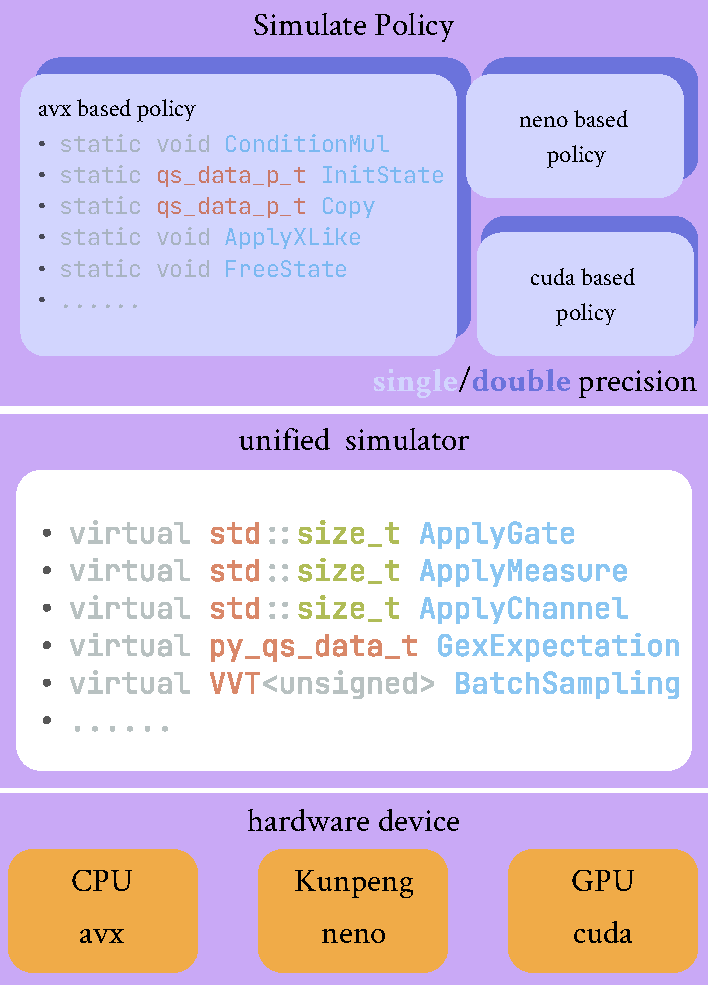
\includegraphics[scale=0.6]{./images/3_1_simulator_structure.pdf}
    \captionsetup{justification=raggedright,singlelinecheck=false}
    \caption{\label{3_1_sim_str} 模拟器的层级结构。\textit{simulate policy} 层根据当前模拟硬件将量子门作用到量子态上。\textit{unified simulator} 层使用不同策略完成线路模拟、期望值计算和梯度计算。\textit{hardware device} 层展示了我们对 CPU、GPU 和鲲鹏平台的支持。}
\end{figure}

根据所模拟的具体量子系统，可以选择全振幅量子模拟器或密度矩阵模拟器。在 \MindQuantum\ 中，这两种模拟器分别称为 \code{"mqvector"} 和 \code{"mqmatrix"}。在当前 \version\ 版本中，\code{"mqvector"} 模拟器也支持 GPU 加速，并命名为 \code{"mqvector_gpu"}。\code{"mqvector"} 和 \code{"mqmatrix"} 都采用图~\ref{3_1_sim_str} 所示的相同设计模式。基于这些模拟器，还可以借助量子信道支持噪声模拟，这将在第~\ref{sec:noise_simulation} 节中讨论。

\subsubsection{基于 SIMD 的量子门优化}
SIMD（Single Instruction Multiple Data，单指令多数据）是一种计算机架构和并行处理技术，旨在通过同时对多个数据元素施加同一操作，加速可并行化任务的执行。量子模拟器的基本构件是量子门与量子态之间的相互作用，其中涉及大量并行操作，因此可以利用 SIMD 提升量子模拟速度。本节将展示如何在 \code{complex128} 数据类型下，基于 AVX 指令优化量子门演化。

AVX 指令提供 256 位宽的向量寄存器，可存储 4 个双精度实数或 2 个双精度复数。在图~\ref{fig:avx} 中，我们以二量子比特全状态矢量为例，概率振幅 $a$ 和 $b$ 可以同时加载到一个 256 位寄存器中，$c$ 和 $d$ 也可以同样处理。
\begin{figure}
    \begin{tikzpicture}[scale=0.5]
        \node[left] at (0,0.5) {256 位寄存器};
        \draw[line width=1.2] (0,0) rectangle (1, 1);
        \draw[line width=1.2] (1,0) rectangle (2, 1);
        \draw[line width=1.2] (2,0) rectangle (3, 1);
        \draw[fill=black] (3.6, 0.5) circle (0.1);
        \draw[fill=black] (4.0, 0.5) circle (0.1);
        \draw[fill=black] (4.4, 0.5) circle (0.1);
        \draw[line width=1.2] (5,0) rectangle (6, 1);
        \draw[line width=1.2] (6,0) rectangle (7, 1);
        \draw[line width=1.2] (7,0) rectangle (8, 1);
        \node[left] at (0,-1) {寄存器 a};
        \draw[line width=1.2] (0,-1.5) rectangle (2, -0.5);
        \draw[line width=1.2] (2,-1.5) rectangle (4, -0.5);
        \draw[line width=1.2] (4,-1.5) rectangle (6, -0.5);
        \draw[line width=1.2] (6,-1.5) rectangle (8, -0.5);
        \node at (1,-1) {$b_i$};
        \node at (3,-1) {$b_r$};
        \node at (5,-1) {$a_i$};
        \node at (7,-1) {$a_r$};
        \node[left] at (0,-2.5) {寄存器 b};
        \draw[line width=1.2] (0,-3) rectangle (2, -2);
        \draw[line width=1.2] (2,-3) rectangle (4, -2);
        \draw[line width=1.2] (4,-3) rectangle (6, -2);
        \draw[line width=1.2] (6,-3) rectangle (8, -2);
        \node at (1,-2.5) {$d_i$};
        \node at (3,-2.5) {$d_r$};
        \node at (5,-2.5) {$c_i$};
        \node at (7,-2.5) {$c_r$};
        \draw[dashed, line width=1.2, fill=red!50] (8, -0.5) -- (8, -1.5) -- (10, -1.4) -- (12, -1.4) -- (12, 0.5) -- (10, 0.5) -- cycle;
        \draw[dashed, line width=1.2, fill=blue!50] (8, -2) -- (8, -3) -- (10, -3.4) -- (12, -3.4) -- (12, -1.6) -- (10, -1.6) -- cycle;
        \node[right] at (9, 1) {$\ket{\psi}=$};
        \node[right] at (9.5, -0) {$a\ket{00}+$};
        \node[right] at (9.5, -1) {$b\ket{01}+$};
        \node[right] at (9.5, -2) {$c\ket{10}+$};
        \node[right] at (9.5, -3) {$d\ket{11}$};
    \end{tikzpicture}
    \caption{将二量子比特量子态存储到两个 256 位寄存器中。}
    \label{fig:avx}
\end{figure}

我们将基本量子门划分为不同类型，例如类 X 门、类 Z 门或矩阵门。对于类 X 门，矩阵元素仅位于反对角线上：
\begin{equation}
    \begin{pmatrix}
        0 & a \\
        b & 0
    \end{pmatrix}.
\end{equation}
当类 X 门作用在第一个量子比特上时，需要在单个 AVX 寄存器中交换 $(b*a_r, b*a_i)$ 和 $(a*b_r, a*b_i)$。如果该门作用在其他量子比特上，则需要交换 $b*\text{reg\_a}$ 和 $a*\text{reg\_b}$。对于类 Z 门，矩阵元素仅位于对角线上：
\begin{equation}
    \begin{pmatrix}
        a & 0 \\
        0 & b
    \end{pmatrix}.
\end{equation}
在这种情况下，如果量子门作用在第一个量子比特上，只需将 $(a_r, a_i)$ 改为 $(a*a_r, a*a_i)$，并将 $(b_r, b_i)$ 改为 $(b*b_r, b*b_i)$；如果作用在其他量子比特上，则只需让寄存器 a 乘以 $a$，寄存器 b 乘以 $b$。

\subsection{密度矩阵模拟器}
不同于状态矢量模拟器，密度矩阵模拟器更适合混态或开放量子系统模拟，但内存消耗也大得多。量子系统的密度算符描述为：
\begin{equation}
    \rho=\sum_ip_i\ket{\psi_i}\bra{\psi_i},
\end{equation}
其中，$p_i$ 是系统处于纯态 $\ket{\psi_i}$ 的概率。量子门 $U$ 对密度算符的演化为：
\begin{equation}
    \rho'=U\rho U^\dagger.
\end{equation}
可观测量 $H$ 在 $\rho$ 下的期望值为：
\begin{equation}
    \left<H\right> = \sum_ip_i\bra{\psi_i}H\ket{\psi_i}=\tr(\rho H).
\end{equation}

其使用方法、开发策略和优化流程都与状态矢量模拟器非常相似，请参见第~\ref{sec_state_vec} 节。
